\documentclass[style=upen, size=14pt]{powerdot}
\usepackage{natbib}
\usepackage{bibentry}
\usepackage{mathtools}
\definecolor{arany}{RGB}{255,242,0}
\hypersetup{backref=page}
\hypersetup{
    colorlinks=true,
    linkcolor=cyan,
    citecolor=cyan,
    filecolor=magenta,      
    urlcolor=cyan}
% \pdsetup{trans=Split}
\usepackage{graphicx}
\usepackage{amsmath}
\DeclareMathOperator*{\argmax}{argmax}
\DeclareMathOperator*{\argmin}{argmin}
\DeclareMathOperator*{\softmax}{softmax}
\DeclareMathOperator{\sign}{sign}
\usepackage{amssymb}
\usepackage{stmaryrd}
\usepackage[latin2]{inputenc}
%\usepackage[magyar]{babel}
%\usepackage{euler}
\usepackage{tikz}
\usetikzlibrary{matrix}
%\usepackage{tikz-qtree}
%\usepackage{tikz-dependency}
%\usepackage{linguex}
\usepackage{amsthm}
\usepackage{amsmath}
%\tikzset{every tree node/.style={align=center,anchor=north}}
%\usepackage{tabularx}
%\usepackage{threeparttable}
%\usepackage{color}
%\selectlanguage{english}
%\frenchspacing
\usepackage{algpseudocode}
\usepackage{algorithm}
\newcommand\varlist{,\makebox[1em][c]{.\hfil.\hfil.},}
\newcommand{\nd}{\noindent}
\newcommand{\Val}{\mathop{\mathit{Val}}}
\newcommand{\gold}{\color{arany}}
%\usepackage{tikz}
%\usepackage{tikz-qtree}
%\newcommand{\qed}{\hfill\mbox{\raggedright \rule{.1in}{.1in}}}
\def\es{\mathbin\land}
\theoremstyle{definition}
\newtheorem*{definition}{Definition}
\newtheorem{axioma}{Axiom}
\newtheorem{tetel}{Theorem}
\newtheorem{prop}{Proposition}
\newtheorem{lemma}{Lemma}
\begin{document}

\title{Natural Language Processing\\~~\\Lecture 8\\Static neural word embeddings}
% \author{}

\date{2021}
\maketitle

\begin{slide}[toc=Vectors and NNs]{Word vectors and neural networks}
  The success of LSI and LSA showed that distribution based vector
  representations of words can be very useful for NLP tasks in general. In the
  case of neural network NLP models, continuous, dense word representations have
  been especially important, because they
  \begin{itemize} 
  \item can be used as informative and economic representations instead of
    simply one-hot encoding words;
  \item can help decreasing the number of model parameters;
  \item can be learned by neural networks from text corpora in a self-supervised
    manner.
  \end{itemize}
\end{slide}

\begin{slide}[toc=]{Word vectors and neural networks cont.}
  One of the first instances of word vectors learnt by a neural network can be
  found in the neural language model of \cite{bengio2003neural}:
  \begin{center}
  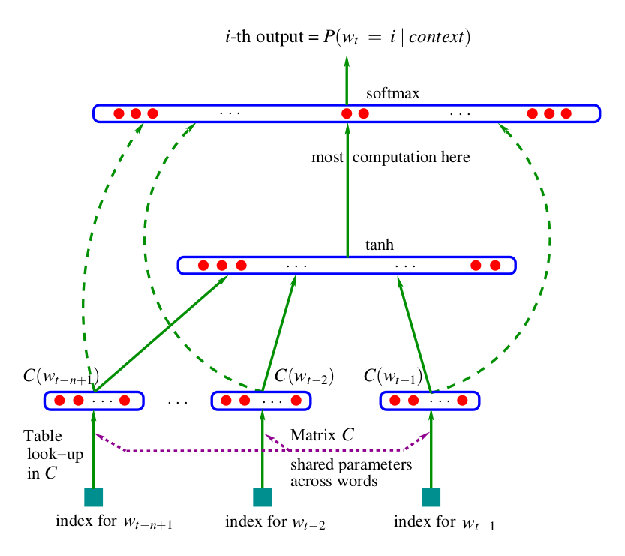
\includegraphics[width=0.6\textwidth]{figures/neural_lm.eps}
  \end{center}
\end{slide}

\begin{slide}[toc=]{Word vectors and neural networks cont.}
  $C$ is an embedding layer mapping word vocabulary indexes to vectors of real
  numbers:
  $$
  C: [0, |V|)  \rightarrow \mathbb R^d.
  $$
  The $d$ dimensionality of (static) word embeddings is typically within the
  50--600 range.

  Technically, embedding layers can be implemented in several ways, e.g., as a
  dense layer with one-hot encoded word indexes as input (in this case the word
  vectors are represented as the weight matrix of the layer), or as a look-up
  table represented as an array etc.
\end{slide}

\begin{slide}[toc=]{Word vectors and neural networks cont.}
  Important lessons regarding the embedding layer in \cite{bengio2003neural}:
  \begin{itemize}
  \item Embeddings are \emph{static}: tokens of the same type have identical
    embeddings regardless of their context.
  \item The model using the end-to-end trained word embedding layer performed
    better than traditional \emph{n}-gram based language models.
  \item Using the first principal components of the word co-occurrence frequency
    matrix as word feature vectors instead of the trained embeddings did not
    have the same performance benefits.
  \item Learning word embeddings with neural nets is a viable way of scaling up
    the training corpus. 
  \end{itemize}
\end{slide}

\section{Word2vec}

\begin{slide}[toc=Novelties]{Distinguishing features}
  Word2vec, introduced by \cite{mikolov2013efficient}, is also a neural network
  family learning useful distributed representations of words from a corpus, but
  with several novel features:
  \begin{itemize}
  \item It is a dedicated architecture: \emph{representation learning} is its
    sole goal.
  \item It is based on a new type of corpus-based, self-supervised predictive
    task.
  \item The architecture is kept intentionally very simple to make it possible
    to train on huge corpora with large vocabularies.
  \end{itemize}
\end{slide}

\begin{slide}[toc=Skipgrams]{Skipgrams}
  Word2vec is based on \emph{skipgrams}, which are a generalization of
  $n$-grams: while an $n$-gram is a \emph{continuos}, $n$-long subsequence of a
  text, skipgrams can contain a certain amount of ``jumps'': If the base
  sequence is $\langle w_1\varlist w_N\rangle$ then the set of $n$-long
  skipgrams with at most $k$ total distance is
  $$
  \{\langle w_{i_1} \varlist w_{i_n}\rangle~|~ i_1\varlist i_n\in[1, N],
  \sum_{j=2}^n i_j-i_{j-1} \leq k \}.
  $$
  There can be additional restrictions, e.g. on the number and length of
  individual skips.
\end{slide}

\begin{slide}[toc=Tasks]{Word2vec tasks}
  The Word2vec task is specifically based on skipgrams of length $2c$ with a
  single one-word skip at the center. There are two task-variants with
  associated model architectures:
  \begin{itemize}
  \item \emph{\gold CBOW} (Continuous Bag of Words): predict the missing word at
    the center of a skipgram. 
  \item \emph{\gold SkipGram}: predict the elements of the skipgram given the
    missing/skipped word. In contrast to the CBOW task, where each skipgram
    corresponds to exactly one classification example, the SkipGram task
    produces several $\langle$word-in-the-center word-from-the-skipgram$\rangle$
    examples for each skipgram.
  \end{itemize} 
\end{slide}

\begin{slide}[toc=]{Word2vec tasks cont.}
  A simple illustration of the skipgram task:
  \begin{center}
    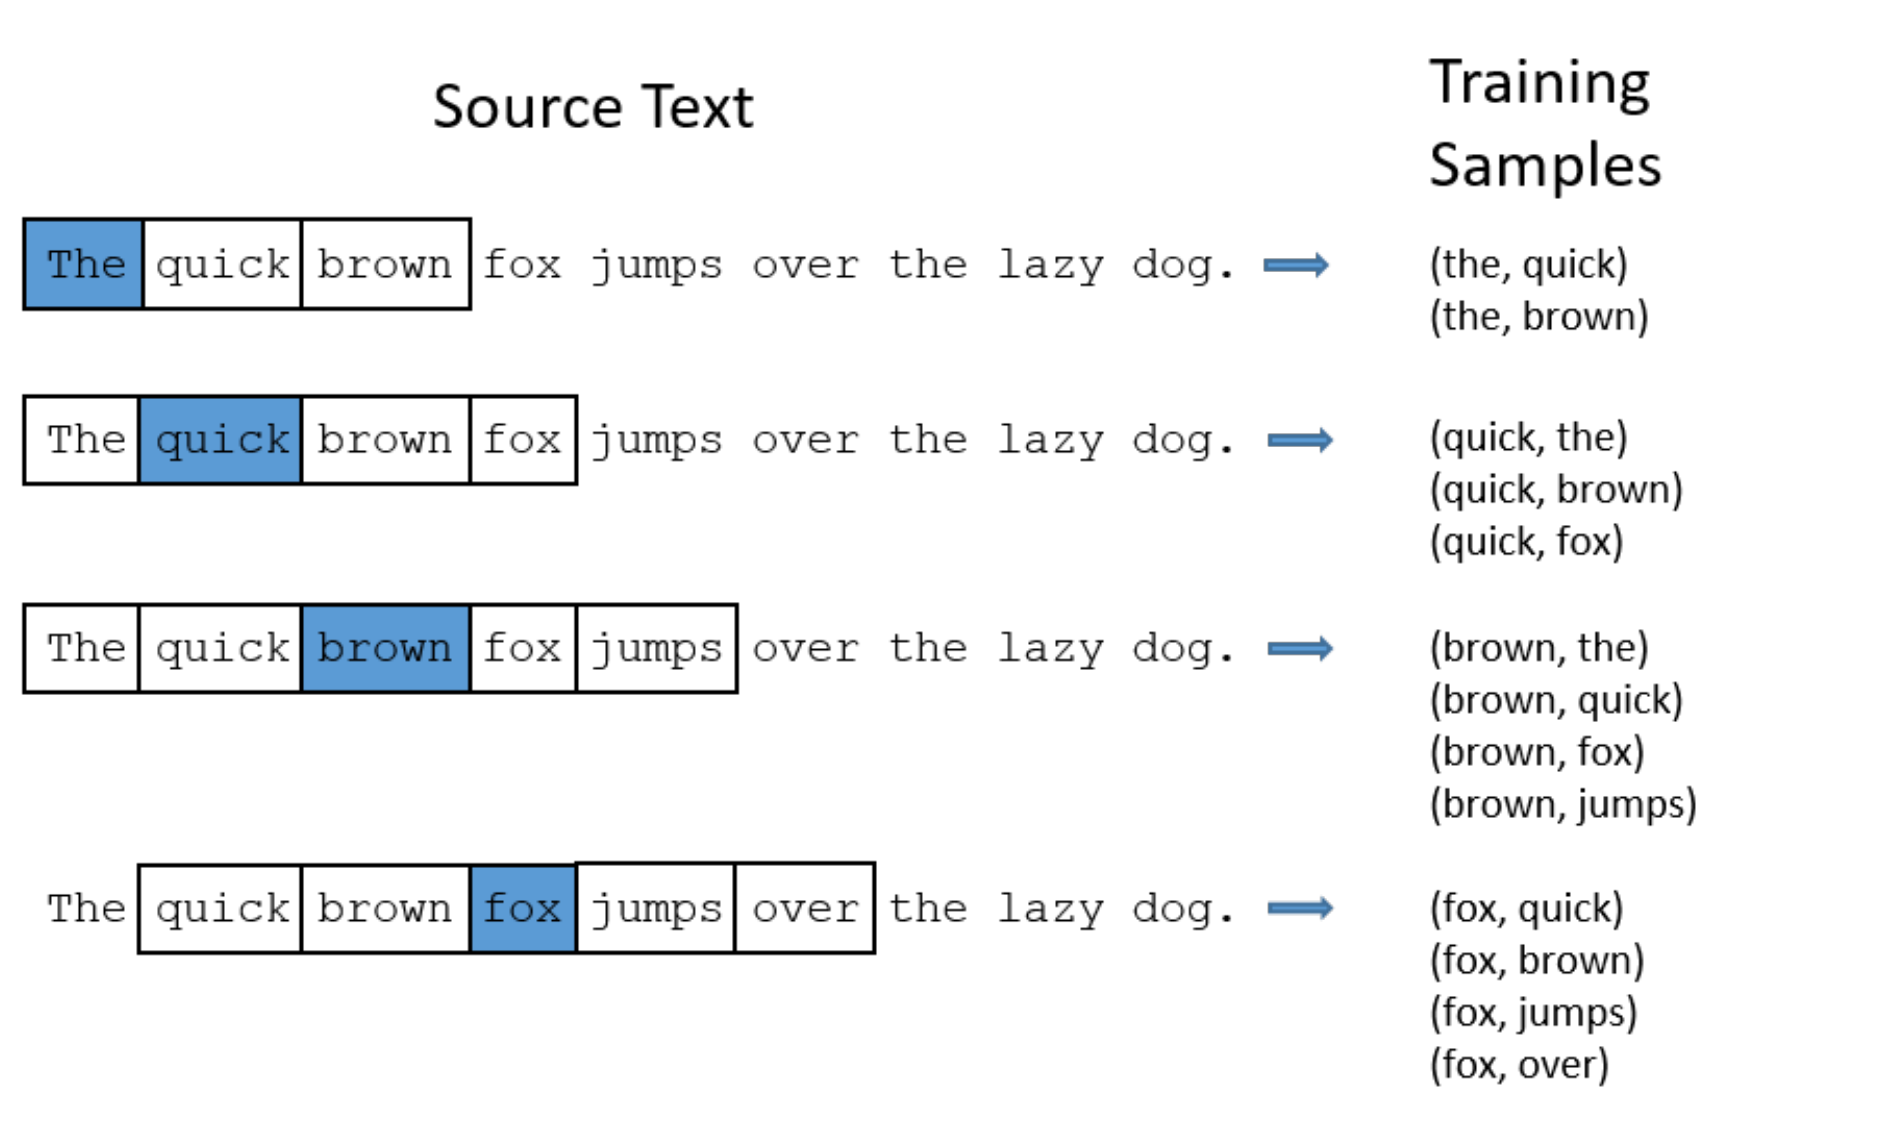
\includegraphics[width=0.9\textwidth]{figures/skipgram.eps}
    \footnotesize{(Figure from \href{http://mccormickml.com/2016/04/19/word2vec-tutorial-the-skip-gram-model/}{McCornick: Word2vec tutorial})}
  \end{center}  
\end{slide}

\begin{slide}[toc=Architecture]{Architecture}
  \begin{center}
    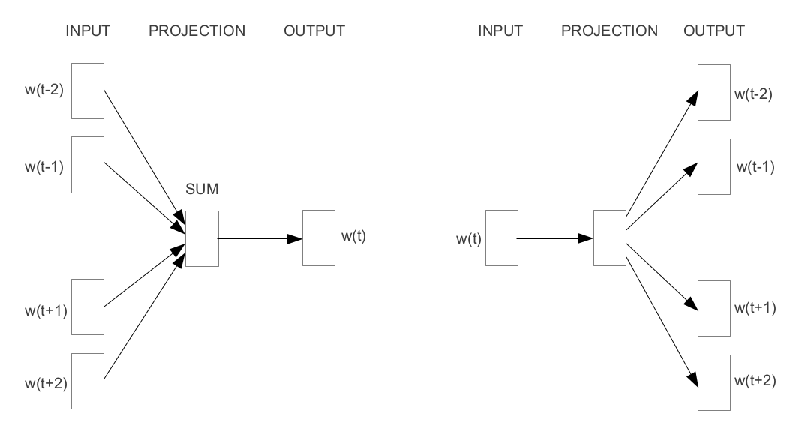
\includegraphics[width=0.8\textwidth]{figures/w2v_arch.eps}
  \end{center}
  While SkipGram simply applies the $E(\cdot)$ embedding mapping to its one-word
  input, CBOW embeds all words in the input skipgram and computes their sum.
  % \parbox{1.1\textwidth}{ \parbox{0.6\textwidth}{
  % text here 
  %   \parbox{{0.4\textwidth}}{
  %     \includegraphics[width=0.4\textwidth]{figures/w2v_cbow.eps}} }
\end{slide}

\begin{slide}[toc=]{Architecture cont.}
  After projecting the input into the word embedding space, both architectures
  use simply a linear projection with weight matrix
  $W \in \mathbb R^{|V|\times d}$ and a final softmax layer to produce
  prediction probabilities for all words in the vocabulary:
   
  \begin{small}
  $$
  CBOW(\langle w_{t-c}\varlist w_{t+c} \rangle) = \softmax(W\sum_{i}E(w_i)),
  $$
  $$
  SkipGram(w_t) = \softmax(W_{}E(w_t)).
  $$
  \end{small}

  Both models are trained with standard negative log likelihood loss and SGD,
  but there are interesting differences regarding the sampling of examples.
\end{slide}

\begin{slide}[toc=]{Architecture cont.}
  It is worth noting that the $W \in \mathbb R^{|V|\times d}$ projection matrix
  can also be seen as an $E'(\cdot)$ embedding of the vocabulary into the same
  $R^d$ space. With this notation, the logits (linear outputs) of the two
  models for a particular $w_j$ word can be written simply as
  \begin{small}
  $$
  CBOW_{linear}(\langle w_{t-c}\varlist w_{t+c} \rangle)[w_j] = \sum_{i}E(w_i) \cdot E'(w_j),
  $$
  $$
  SkipGram_{linear}(w_t)[w_j] = E(w_t) \cdot E'(w_j)
  $$
\end{small}
As this formulation shows, minimizing the negative log likelihood training
objective is a way of increasing the dot product of the embeddings of the input
and that of the correct prediction.
\end{slide}

\begin{slide}[toc=]{Architecture cont.}
  Because of the symmetry shown by this formulation, it is an option to
  \emph{tie the weights} of the two layers making $E(w) = E'(w)$ for all
  $w\in V$.

  Although this is frequently done, it's also customary to keep them different
  and only use the vectors of the input embedding $E(\cdot)$ as the final result, or
  combine them, e.g., by taking their average.
\end{slide}

\begin{slide}[toc=Data generation]{Data point generation and sampling}
  For the CBOW variant, we simply slide the $c$-radius context window through
  the corpus and generate a 
  $$\langle \langle w_{t-c}\varlist w_{t-1}, w_{t+1}\varlist w_{t+c} \rangle, w_t \rangle$$
  $\langle$input, correct output$\rangle$ data point at each step.\bigskip

  The process is more complicated for SkipGram, because at each step the
  actually used context window radius $r$ is randomly chosen from the $[1, c]$
  interval, and a $\langle w_t, w_i\rangle$ data point is generated for each
  $w_i\in \langle w_{t-r}\varlist w_{t-1}, w_{t+1}\varlist w_{t+r}\rangle$ word.
  The effect is that words closer to the target are sampled with a higher
  probability.
\end{slide}

\begin{slide}[toc=Softmax alternatives]{Avoiding full softmax}
  As computing full softmax for a $|V|$-long vector is expensive for large $V$s,
  Word2vec implementations typically use cheaper output layer
  alternatives.\bigskip

  One solution is \emph{\gold hierarchical softmax}, which is based on a binary
  tree whose leaves are the vocabulary words. The linear outputs of the network
  correspond to internal nodes, and the probability assigned to a $w$ word can
  be calculated by computing values of $\sigma(o)$ only for the $o$ outputs that
  lie on the path to $w$. Using a balanced tree this trick reduces the softmax
  computation complexity during training from $\mathcal O(|V|)$ to
  $\mathcal O({\log |V|})$, and with clever tree structure this can be further
  decreased.
\end{slide}

\begin{slide}[toc=]{Hierarchical softmax}
  \begin{center}
    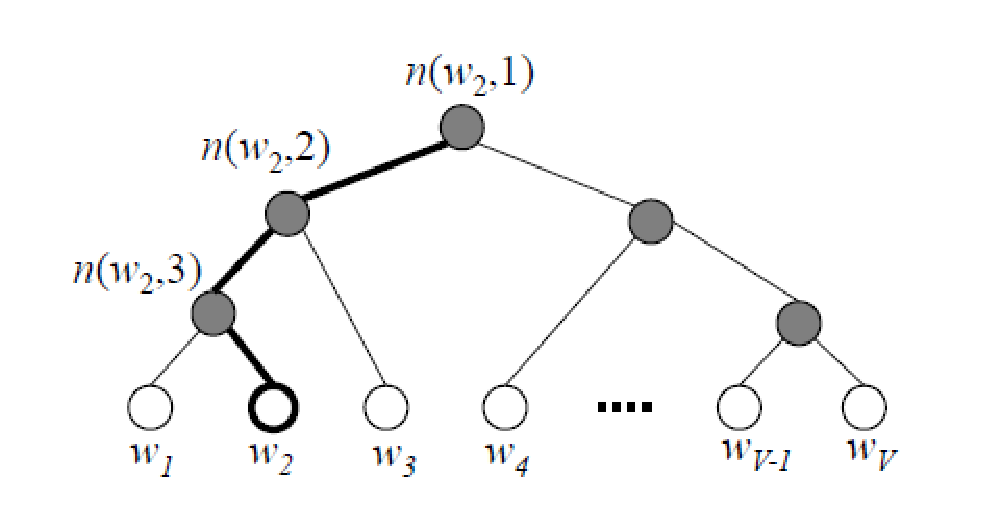
\includegraphics[width=0.65\textwidth]{figures/hierarchic_softmax.eps}
\end{center}
Illustration: if the linear outputs on the path are $o(w_2, 1), o(w_2, 2), o(w_2, 3)$ then the
probability assigned to $w_2$ can be calculated as
$(1-\sigma(o(w_2,1)))(1-\sigma(o(w_2,2)))\sigma(o(w_2,3))=
\sigma(-o(w_2,1))\sigma(-o(w_2,2))\sigma(o(w_2,3))$.
\end{slide}

\begin{slide}[toc=]{Negative sampling}
  The other alternative is \emph{\gold negative
    sampling}\footnote{\citet{mikolov2013distributed}.} This involves
  reformulating the SkipGram task as a binary classification problem.
  \begin{itemize}
  \item We consider earlier SkipGram $\langle$center word, context word$\rangle$
    data points from the corpus as positive examples,
  \item and also generate a certain number of negative examples by sampling, for
    each center word, ``fake context words'' from a noise distribution
    representing the entire corpus.
  \end{itemize}
\end{slide}

\begin{slide}[toc=]{Negative sampling}
  The negative sampling trick makes it possible to simplify the network
  architecture to the point of
  $$
  SGNS(w_{t}, w_{c}) = \sigma(E_t(w_t)\cdot E_c(w_c)) 
  $$
  where $E_t(\cdot)$ is the target (center) word embedding while $E_c(\cdot)$ is
  the context word embedding. With $k$ negative samples from a $P_n$ noise
  distribution, the negative log likelihood loss for each real
  $\langle w_t, w_c\rangle$ data point will be
  $$
  - [ \log SGNS(w_{t}, w_{c}) + \sum_{\substack{i=1 \\ {w}_c \sim P_n}}^k
  \log(1 - SGNS(w_{t}, {{w}_c}))].  $$
\end{slide}

\begin{slide}[toc=W2V as factorization]{Word2vec as matrix factorization}
  After the success of Word2Vec, many studies investigated its relationship to
  counting based matrix factorization methods, and they turned out to be closely
  related: \cite{levy2014neural} showed that the SGNS objective is equivalent to
  factorizing the word co-occurrence based $M$ matrix whose elements are

  $$
  m_{ij} = \max(0, PMI(w_i, w_j )- \log k),
  $$
  where $PMI(w_i,w_j)$ is the
  $\frac{P(w_i, w_j)}{P(w_i)P(w_j)}\approx \frac{C(w_i, w_j)}{C(w_i)C(w_j)}$
  \emph{pointwise mutual information} of $w_i$ and $w_j$, and $k$ is the number
  of negative samples.
\end{slide}

\section{GloVe}


\begin{slide}[toc=Algorithm]{The GloVe algorithm}
  \emph{\gold GloVe} (Global Vectors)\footnote{\cite{pennington2014glove}.} is
  another algorithm for learning static word embeddings from a very large
  corpus. It is \emph{not} a neural method, but discussed here because it was
  published (one year) after Word2vec as a reaction to it, and is one of its
  most important alternatives.\bigskip

  Similarly to LSA methods, GloVe is explicitly based on a low-rank
  factorization of a matrix based on word-occurrences in fixed-size context
  windows, but the matrix elements are actually the \emph{logarithms} of word
  co-occurrences.
\end{slide}

\begin{slide}[toc=]{The GloVe algorithm cont.} 
  Focusing on the logarithm of co-occurrences is motivated by the observation
  that \emph{ratios} of co-occurrence probabilities are very informative
  semantically:
  \begin{center}
    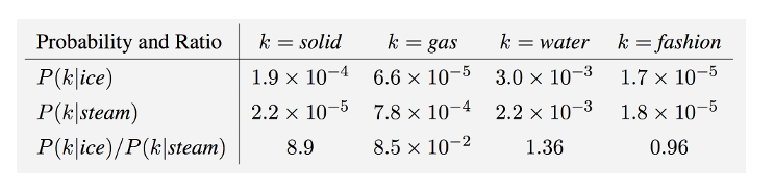
\includegraphics[width=0.9\textwidth]{figures/glove.eps}
  \end{center}
  The table shows that the ratios do a good job in distinguishing words that are
  relevant to the word pair \emph{ice}, \emph{steam}, i.e., \emph{solid} and
  \emph{gas} from noise words.
\end{slide}

\begin{slide}[toc=]{The GloVe algorithm cont.} 
  Factorizing directly the co-occurrence log probability matrix would require
  for any $w_i$, $w_j$ word pair
  \begin{small}
    $$
    E_w(w_i)\cdot E_c(w_j)\approx \log (P(w_j~|~ w_i)) \approx \log (C(w_i, w_j)) - \log (C(w_i)).
    $$
  \end{small}
  With $E_w(\cdot)$ word and $E_c(\cdot)$ context embeddings satisfying this
  requirement the $\log(P(w_k~|~w_i)/P(w_k~|~w_j))$ log probability ratio can be
  expressed simply as

  $(E_w(w_i) - E_w(w_j))\cdot E_c(w_k)$, i.e., the semantically informative
  co-occurrence relationships correspond to simple geometric ones between the embeddings.
\end{slide}

\begin{slide}[toc=]{The GloVe algorithm cont.}
  Instead of trying to minimize the differences
  $E_w(w_i) \cdot E_c(w_j) + \log (C(w_i)) - \log (C(w_i, w_j))$ for
  $w_1,w_2\in V$, GloVe minimizes the closely related
  \begin{small}
  $$
  \sum\limits_{i, j=1}^{|V|} f(C(w_i,w_j)) (E_w(w_i)\cdot E_c({w}_j) + b_w(w_i) +
  {b_c}(w_j) - \text{log} C(w_i, w_j))^2
  $$
  \end{small}
  objective. The differences are
  \begin{itemize}
  \item the $f(\cdot)$ weighting function downweighting rare co-occurrences,
  \item the learned $b_w$ and $b_c$ biases for each word, providing a symmetric
    replacement for $\log(C(w_i))$.
  \end{itemize}
\end{slide}

\begin{slide}[toc=]{GloVe Training}
  Unlike Word2vec, which is trained with sliding context windows through the
  corpus, GloVe is trained in two steps:
  \begin{enumerate}
  \item assembling the global co-occurrence counts matrix;
  \item optimizing the $E_w, E_c, b_w, b_c$ parameters in the above objective by
    SGD, randomly sampling the elements of the co-occurrence matrix.
  \end{enumerate}
  Compared to Word2vec, GloVe can have larger memory requirements because of
  working with the co-occurrence matrix (although it is sparse), but this can be
  compensated by the fact that optimization happens on the non-zero matrix
  elements afterwards, whose number is typically sublinear in corpus length.
\end{slide}

\section{Evaluation}

\begin{slide}[toc=Evaluation types]{Types of evaluation}
  How can the quality of word embeddings be measured? As learned
  representations, word vectors can be evaluated
  \begin{itemize}
  \item \emph{\gold intrinsically}, according to how well they correspond to
    human judgments about the semantic and morphological features of words, and
  \item \emph{\gold extrinsically}, according to how useful they are as
    components in solutions of downstream NLP tasks.
  \end{itemize}
  As for the intrinsic point of view, Word2vec with appropriately fine-tuned
  parameters and on a large, good quality corpus can produce embeddings whose
  geometrical characteristics are surprisingly close to human similarity
  judgments.
\end{slide}

\begin{slide}[toc=Intrinsic]{Intrinsic evaluation}
  The two most used intrinsic metrics are
  \begin{itemize}
  \item how well the \emph{\gold cosine similarity} of two representations,
    $\frac{E(w_1)\cdot E(w_2)}{\|E(w_1)\|\times \|E(w_2)\|} $, correlates with
    human-assigned similarity scores;
  \item how well similar \emph{\gold relationships} between words, e.g,.
    $king:queen$ and $man:woman$ correspond to similar geometric relationships
    between the vectors. It is typical to look at the \emph{difference} between
    the vectors, i.e., whether $E(king)-E(queen)\approx E(man)-E(woman)$, or, in
    a slightly different formulation, whether the word whose embedding is the
    closest to $E(king)-E(queen) + E(woman)$ is $man$.
  \end{itemize}
\end{slide}

\begin{slide}[toc=]{Intrinsic evaluation cont.}
  These intrinsic metrics can be nicely visualized using dimension reduction
  techniques such as t-SNE or UMAP, e.g., 
  \begin{center}
    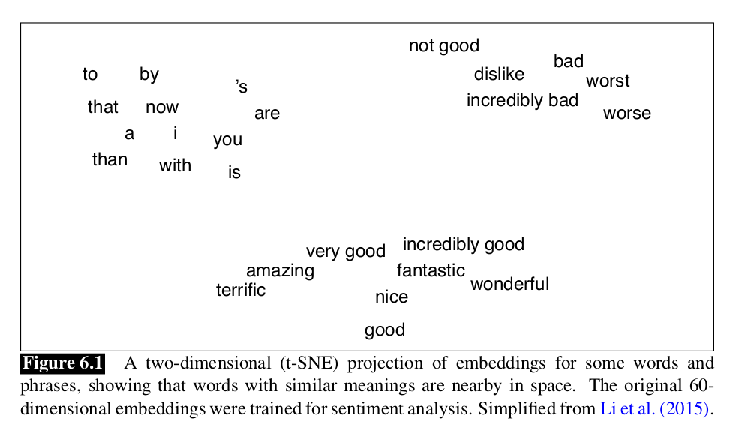
\includegraphics[width=0.8\textwidth]{figures/w2v_tsne.eps}
    
    (\footnotesize Figure from \citet[ch. 6]{jurafsky2019speech}.)
  \end{center}  
\end{slide}

\begin{slide}[toc=]{Intrinsic evaluation cont.}
  There are also purpose built \emph{datasets} for intrinsic evaluation, e.g.,
  \begin{itemize}
  \item the
    \href{http://alfonseca.org/eng/research/wordsim353.html}{WorsSim-353}
    dataset containing 353 English word pairs with semantic similarity scores
    between 1.0 and 10.0;
  \item \href{https://vecto.space/projects/BATS/}{BATS} (The Bigger Analogy Test
    Set) containing 98000 analogy questions for testing the correspondence
    between word analogies and vector offsets.
  \end{itemize}
\end{slide}

\begin{slide}[toc=Extrinsic]{Extrinsic evaluation}
  Extrinsic evaluation can be performed using any NLP task, but it is typical to
  use standard sequence labeling tasks such as named entity recognition.

  Embeddings can be evaluated by switching between them in an embedding-based
  architecture while keeping everything else fixed.\bigskip

  There is an important difference between using the embeddings ``as is''/``frozen''
  without changing them, or \emph{\gold fine tuning} them, i.e., training them
  on the task dataset together with the other parameters.
\end{slide}

\begin{slide}[toc=Results]{Evaluation results}
  According to the intrinsic evaluation results of \cite{levy2015improving},
  there is no large difference in performance between Word2vec variants, GloVe
  and traditional SVD on certain co-occurrence matrixes. Most importantly, they
  found that
  \begin{itemize}
  \item hyperparameter tuning influences performance more than the choice of algorithm,
  \item SGNS proved to be a very strong baseline which did not ``significantly
    underperform in any scenario'',
  \item the \emph{sum} of the two learned embeddings (target and context) often
    performs significantly better than only one of them.
  \end{itemize}
\end{slide}

\section[toc=Internal word structure]{Utilizing internal word structure}

\begin{slide}[toc=Blackbox problem]{The blackbox problem}
  The word embeddings we have discussed so far are based \emph{exclusively} on
  distribution, the \emph{internal structure} of words do not play any role.
  Consequently,
  \begin{itemize}
  \item out of vocabulary words, and
  \item words that are rare in the training corpus
  \end{itemize}
  do not have adequate embeddings, even if their internal
  morphological/character structure could provide ample information about their
  semantic and syntactic properties.\bigskip

  Apart from using \emph{morpheme} embeddings, which requires a morphological
  analyser, a few self-supervised solutions also emerged.
\end{slide}

\begin{slide}[toc=fastText]{fastText}
  The fastText algoritm \footnote{\cite{bojanowski2017enriching}.} is based on
  SGNS, but adds $n$-grams ($3\leq n \leq 6$) to the vocabulary and models
  target words as the sum of the embeddings of all of its components. E.g., for
  the word \emph{where} and $n=3$ the components are \texttt{<wh}, \texttt{whe},
  \texttt{her}, \texttt{ere}, \texttt{re>}, plus the whole word
  \texttt{<where>}. The SGNS architecture is modified to 

  $$
  \sigma(\sum_{w\in G(w_t)}E_t(w)\cdot E_c(w_c)) 
  $$
  where $G(w_t)$ is the set of all components of $w_t$.
\end{slide}

\begin{slide}[toc=]{fastText cont.}
  On similarity tasks fastText vectors typically perform better than vanilla
  Word2vec, especially in case of morphologically rich languages.\bigskip

  An additional, important advantage is that with fastText it is possible to
  generate informative embeddings for unseen words by summing up the embeddings
  of their component $n$-grams.
\end{slide}

\begin{slide}{Subword embeddings}
  A more radical solution to the blackbox problem is to switch to subword
  tokenization (e.g., using BPE) and generate embeddings only for the subwords
  in the vocabulary with one of the established algorithms.\bigskip

  \href{https://github.com/bheinzerling/bpemb}{PBEmb}, for instance, uses GloVe
  to generate embeddings for the subwords resulting from BPE-based tokenization.
  Similarly to fastText, embeddings for OOV words can produced by combining the
  embeddings of component subwords (e.g., averaging them).
  \cite{heinzerling2017bpemb} found that while performing similarly, this type
  of solution requires a markedly smaller vocabulary than fastText.
\end{slide}

\section{References}

\begin{slide}{References}
  \bibliographystyle{plainnat}
  \nobibliography{nlp_course.bib}
  \begin{footnotesize}
    
    \bibentry{bengio2003neural}\medskip

    \bibentry{bojanowski2017enriching}\medskip

    \bibentry{heinzerling2017bpemb}\medskip

    \bibentry{jurafsky2019speech}\medskip

    \bibentry{levy2014neural}\medskip
  
    
  \end{footnotesize}
\end{slide}

\begin{slide}[toc=]{References cont.}
  \begin{footnotesize}

    \bibentry{levy2015improving}\medskip

    \bibentry{mikolov2013efficient}\medskip 

    \bibentry{mikolov2013distributed}\medskip
    
    \bibentry{pennington2014glove}\medskip
    
  \end{footnotesize}
\end{slide}


\end{document}



%%% Local Variables:
%%% mode: latex 
%%% TeX-master: t
%%% End:

% LocalWords:  Tokenization Discriminative discriminative
